\chapter{Análisis Estratégico y de Competencias}

El estado del arte desarrollado en la sección 3 relevó el ecosistema de herramientas analíticas disponibles para el comercio electrónico y permitió identificar, mediante comparación directa con antecedentes concretos, la brecha metodológica que este proyecto busca cubrir. Ese relevamiento, sin embargo, describe el panorama competitivo sin sistematizar de manera explícita cómo las capacidades internas del proyecto se articulan con las condiciones del entorno para derivar en líneas de acción concretas, ni cuál es la intensidad de las fuerzas competitivas que determinan el atractivo de participar en este mercado. El presente capítulo complementa el estado del arte mediante la aplicación de dos herramientas de análisis estratégico de uso extendido en la literatura de administración de empresas: la matriz FODA cruzado, que confronta fortalezas, debilidades, oportunidades y amenazas para generar estrategias concretas \parencite{Weihrich1982}, y el modelo de las cinco fuerzas de Porter, que evalúa la intensidad competitiva del sector \parencite{Porter1979}. Ambos análisis se apoyan, en la medida de lo posible, en evidencia empírica relevada durante las entrevistas realizadas a emprendedores y dueños de comercios PyME, documentadas en el Anexo B, de modo de anclar las conclusiones estratégicas en observaciones concretas del segmento objetivo y no únicamente en apreciaciones teóricas.

\section{Metodología de validación empírica: entrevistas en profundidad frente a encuestas}
\label{sec:metodologia-entrevistas}

La evidencia empírica que sustenta los análisis de este capítulo proviene exclusivamente de entrevistas cualitativas en profundidad, de formato semiestructurado, realizadas a cinco emprendedores y dueños de comercios PyME de los tres rubros objetivo del proyecto (Anexo B). El equipo descartó de manera deliberada el uso de encuestas cuantitativas como instrumento de relevamiento, una decisión que no responde a una limitación de recursos sino a una evaluación explícita de qué instrumento resulta idóneo para el objeto de estudio de este proyecto.

El público objetivo del sistema, dueños de PyMEs y emprendimientos de e-commerce, enfrenta en su operación diaria escenarios de decisión complejos y fuertemente contextuales: el temor al quiebre de stock frente a una demanda que no siempre es predecible, la estacionalidad propia de cada rubro comercial y la fijación de precios en un contexto de inflación e incertidumbre cambiaria. Este tipo de escenario no puede capturarse de forma fehaciente mediante un cuestionario cerrado, que por diseño obliga a reducir situaciones ambiguas y dependientes del contexto a categorías predefinidas por quien lo elabora. Una encuesta hubiese impuesto sobre el fenómeno una estructura de respuesta que el propio relevamiento buscaba, precisamente, descubrir.

Esta limitación se explica, además, por la naturaleza de la pregunta de investigación subyacente. Las encuestas tradicionales son un instrumento adecuado para medir el \enquote{cuánto} o el \enquote{qué}: cuántos comercios llevan un control de stock, qué herramientas utilizan, con qué frecuencia revisan sus precios. Pero el diseño de un sistema de analytics prescriptivo exitoso no podía apoyarse únicamente en esas magnitudes, sino que requería comprender el \enquote{por qué} de cada decisión y, en particular, la carga cognitiva que el comerciante enfrenta al tomarla: qué información tiene disponible en el momento de decidir, qué atajos mentales o heurísticas utiliza ante la incertidumbre, y en qué punto exacto esa carga se vuelve inmanejable y deriva en una decisión postergada o tomada por intuición \parencite{Kahneman2011}. Ese tipo de indagación es, por naturaleza, irreductible a una escala de respuesta cerrada.

El formato semiestructurado aportó, en este sentido, una flexibilidad metodológica que un formulario estático no puede ofrecer: la posibilidad de repreguntar ante una respuesta ambigua, de profundizar en un punto no anticipado por la guía de entrevista original y de adaptar el orden y la formulación de las preguntas al relato particular de cada entrevistado. Esa flexibilidad fue la que permitió descubrir, en la práctica, las soluciones caseras que los comercios del segmento efectivamente utilizan para suplir la falta de herramientas adecuadas, como planillas de Excel compartidas, cuadernos de registro manual o aplicaciones desarrolladas a medida por un conocido, según se documenta en el Anexo B. Ninguna de estas soluciones informales podría haberse anticipado como opción cerrada en un formulario, precisamente porque su existencia era, al momento de diseñar el relevamiento, desconocida para el propio equipo.

Finalmente, el formato de entrevista resultó indispensable para validar empíricamente la disposición a pagar por la herramienta y su sensibilidad al precio, una dimensión que las secciones~\ref{sec:foda-cruzado} y~\ref{sec:porter} retoman en detalle. A diferencia de una pregunta cerrada sobre un rango de precio predefinido, el diálogo en tiempo real permitió observar la reacción espontánea del entrevistado ante la propuesta de valor, repreguntar sobre las condiciones que modificarían esa disposición a pagar y contrastar el monto declarado con el comportamiento efectivo que el propio entrevistado relataba, como la migración hacia plataformas más económicas o la discontinuación de planes pagos ante una percepción de bajo retorno. Esta profundidad conversacional resulta, por definición, inalcanzable para un instrumento cuantitativo cerrado.

Cabe reconocer que esta decisión metodológica implica una limitación conocida: una muestra de cinco entrevistados no permite una generalización estadística al universo de comercios PyME del país. Sin embargo, dado que el objetivo de esta etapa no era medir la magnitud de un fenómeno ya conocido sino explorar y comprender uno todavía poco documentado, la profundidad y el detalle contextual que ofrece la entrevista cualitativa resultan más valiosos, para los fines de este proyecto, que la representatividad estadística que hubiese ofrecido una encuesta con mayor cantidad de respuestas pero de menor riqueza interpretativa.

\section{Design Thinking}
\label{sec:design-thinking}

Como complemento a las entrevistas descriptas en la sección~\ref{sec:metodologia-entrevistas}, el equipo aplicó herramientas de Design Thinking para sintetizar la evidencia cualitativa relevada en artefactos que faciliten la comprensión de las necesidades, motivaciones y frustraciones de los distintos perfiles de usuario, de forma previa a derivar en el análisis estratégico de las secciones siguientes. Esta síntesis no reemplaza el detalle de cada entrevista individual, documentado en el Anexo B, sino que lo condensa en representaciones que permiten identificar patrones comunes y particularidades propias de cada rubro comercial.

\subsection{User Persona}
\label{sec:user-persona}

Se construyeron tres User Personas, personas ficticias que consolidan patrones de comportamiento, motivaciones y frustraciones observados en las entrevistas del Anexo B, una por cada uno de los tres rubros comerciales sobre los que el proyecto focaliza su análisis: indumentaria, gastronomía y electrónica (sección~\ref{sec:comportamiento-consumidor} del Marco Teórico). Esta herramienta permite empatizar con los usuarios e identificar problemáticas específicas según cada perfil, más allá del relato puntual de un único entrevistado.

Lucía Méndez (Figura~\ref{fig:persona-lucia}), del rubro indumentaria, se construyó a partir de las entrevistas a Delfina Fernández y Morena Cejas (Anexo B, Entrevistas B.1 y B.2), ambas emprendedoras de indumentaria que operan sobre Tiendanube y que reconocieron tomar decisiones de reposición y de precio de forma intuitiva, sin apoyo de métricas. Martín Reyes (Figura~\ref{fig:persona-martin}), del rubro gastronomía, se construyó principalmente a partir de la entrevista a Pablo Terrera, dueño de la cafetería MariCafé (Anexo B, Entrevista B.3), quien desarrolló un sistema propio de analytics ante la ausencia de una herramienta del mercado que cubriera su necesidad. Nicolás Acosta (Figura~\ref{fig:persona-nicolas}), del rubro electrónica, constituye una excepción a señalar de forma explícita: ninguno de los cinco entrevistados del Anexo B pertenece a este rubro, por lo que esta persona se construyó a partir de las particularidades descriptas para electrónica en el Marco Teórico (sección~\ref{sec:comportamiento-consumidor}), en particular la desactualización de precios frente a movimientos del tipo de cambio, y de patrones transversales observados en las entrevistas de los otros dos rubros, como la comparación constante de precios y la necesidad de alertas oportunas. Esta distinción se marca para no atribuir a esta persona un respaldo empírico directo del que las otras dos sí disponen.

\begin{figure}[ht]
    \centering
    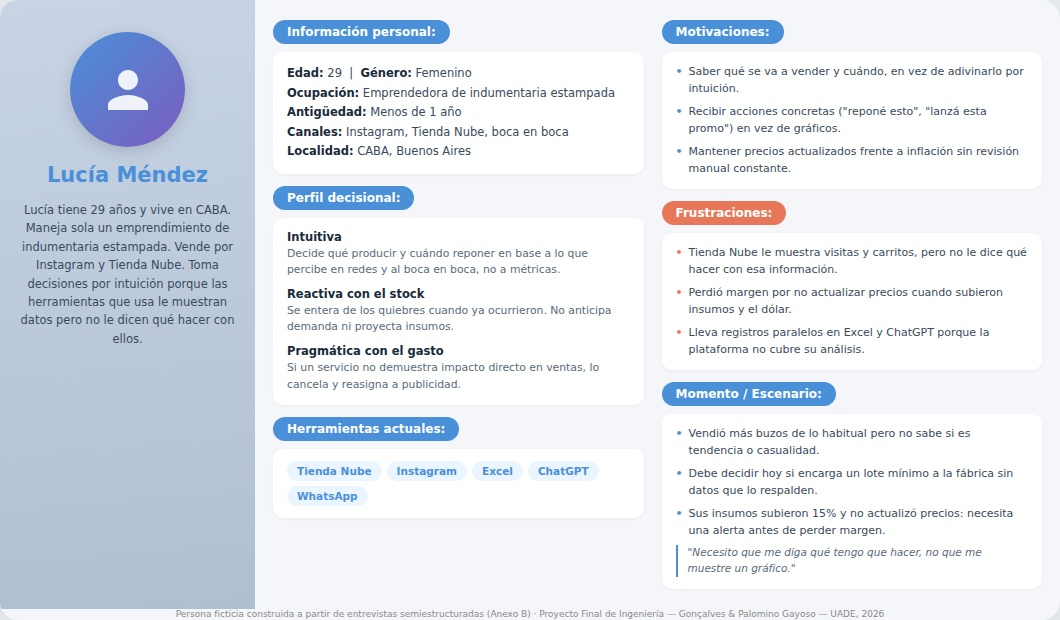
\includegraphics[width=0.85\textwidth]{./images/user-persona-1-lucia-mendez.jpg}
    \caption{User Persona: Lucía Méndez (rubro indumentaria).}
    \label{fig:persona-lucia}
\end{figure}

\begin{figure}[ht]
    \centering
    
\includegraphics[width=0.85\textwidth]{./images/user-persona-2-martin-reyes.jpg}
    \caption{User Persona: Martín Reyes (rubro gastronomía).}
    \label{fig:persona-martin}
\end{figure}

\begin{figure}[ht]
    \centering
    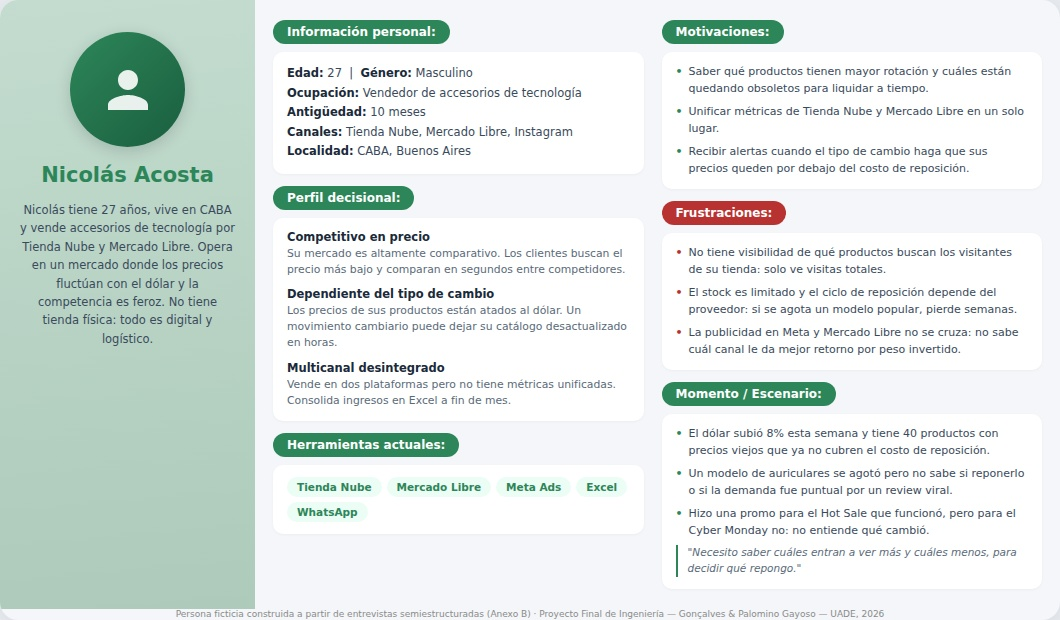
\includegraphics[width=0.85\textwidth]{./images/user-persona-3-nicolas-acosta.jpg}
    \caption{User Persona: Nicolás Acosta (rubro electrónica).}
    \label{fig:persona-nicolas}
\end{figure}

\noindent\textit{Fuente: elaboración propia.}

Las tres personas comparten un mismo diagnóstico de fondo, ya adelantado en la sección~\ref{sec:metodologia-entrevistas}: disponen de datos, propios o de la plataforma que utilizan, pero no de una interpretación accionable de esos datos. Esta necesidad común se retoma de forma directa en las estrategias adaptativas (DO) de la matriz FODA cruzado desarrollada a continuación, orientadas a reducir la barrera de alfabetización analítica del segmento.

\FloatBarrier

\subsection{Mapa de empatía}
\label{sec:mapa-empatia}

Para profundizar en las tres User Personas, se construyó un mapa de empatía por cada una de ellas. Esta herramienta desagrega, en las categorías habituales de \enquote{piensa y siente}, \enquote{ve}, \enquote{escucha}, \enquote{dice y hace}, frustraciones y motivaciones, el contexto emocional y cognitivo en el que cada persona toma sus decisiones, y complementa así las fichas presentadas en la sección~\ref{sec:user-persona}.

El mapa de Lucía Méndez (Figura~\ref{fig:empatia-lucia}), rubro indumentaria, complementa su ficha de persona (Figura~\ref{fig:persona-lucia}). Su construcción permite identificar dos ejes recurrentes: por un lado, una brecha entre lo que Lucía puede intuir, redes sociales y comentarios de otras emprendedoras, y lo que la plataforma le muestra sin traducir en una acción concreta (\enquote{Tienda Nube le muestra estadísticas pero en planes más caros}, \enquote{Gráficos en Tienda Nube que no sabe interpretar}); por otro, un patrón reactivo y no anticipatorio en la gestión de stock (\enquote{Repone stock recién cuando le llega la alerta de quiebre}), consistente con el perfil \enquote{Reactiva con el stock} ya señalado en su ficha de persona.

\begin{figure}[ht]
    \centering
    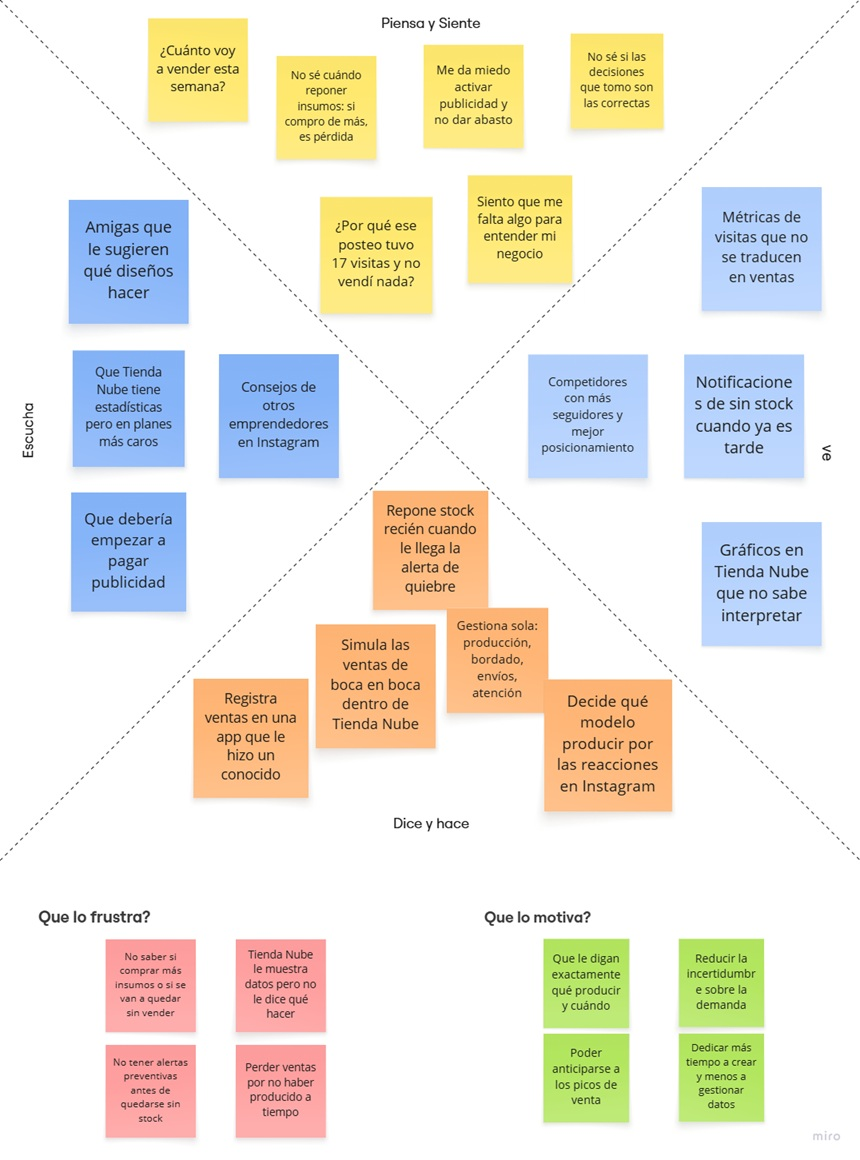
\includegraphics[width=\textwidth]{./images/mapa_empatia_lucia_mendez.jpg}
    \caption{Mapa de empatía: Lucía Méndez (rubro indumentaria).}
    \label{fig:empatia-lucia}
\end{figure}

\noindent\textit{Fuente: elaboración propia.}

\FloatBarrier

El mapa de Martín Reyes (Figura~\ref{fig:empatia-martin}), rubro gastronomía, complementa su ficha de persona (Figura~\ref{fig:persona-martin}) y expone una tensión particular: a diferencia de Lucía, Martín ya construyó una solución propia de analytics combinando Lovable, Google Sheets y Gemini AI (\enquote{La IA puede democratizar lo que hacen las multinacionales}), en línea con el caso real de Pablo Terrera y su sistema Maricapp, documentado en la Sección~\ref{sec:porter}. Esa solución casera, sin embargo, no resuelve dos fricciones que el mapa expone con claridad: la perecibilidad de sus insumos, que no admite margen de error en la reposición (\enquote{Si la crema vence en 20 días, no admite error}), y la sensibilidad de su negocio a variables externas que escapan a cualquier planilla, desde el clima del fin de semana hasta las comisiones de las aplicaciones de delivery y los aumentos de proveedores. Ambas fricciones son consistentes con los rasgos \enquote{Condicionado por perecibilidad} y \enquote{Sensible al contexto macro} ya señalados en su ficha de persona.

\begin{figure}[ht]
    \centering
    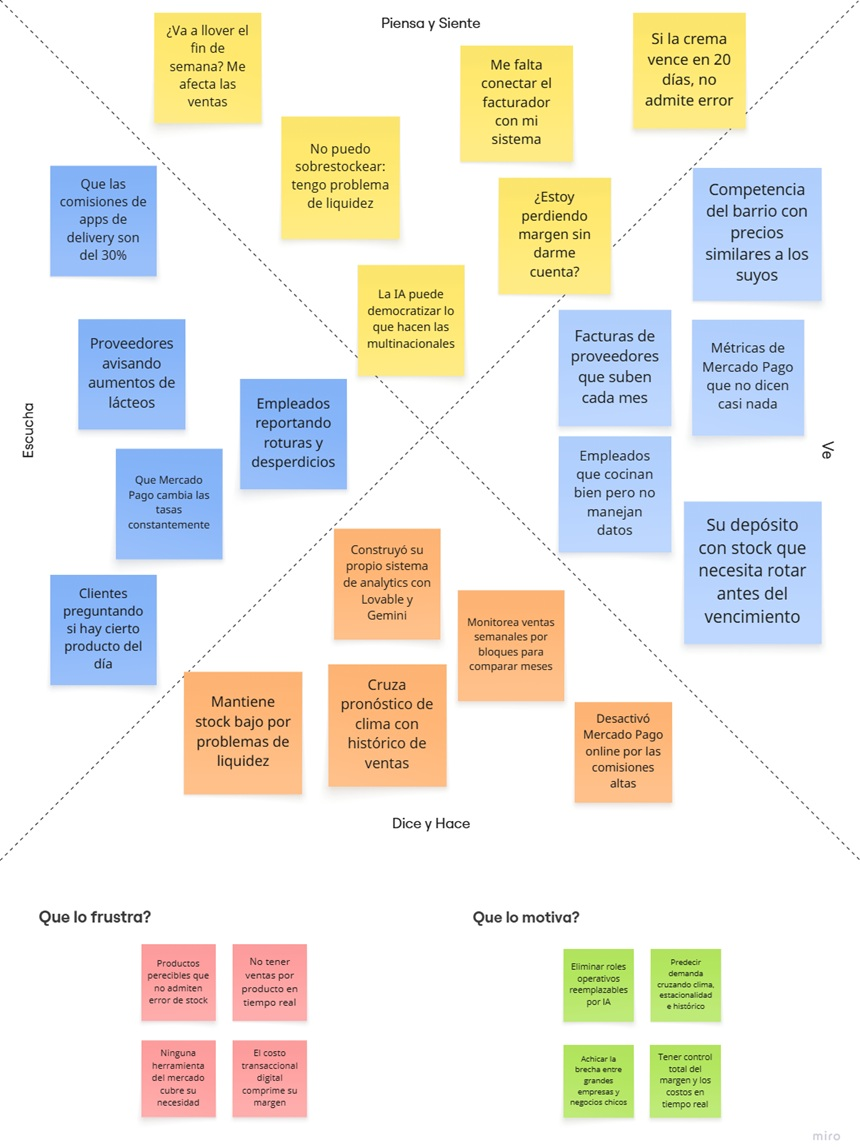
\includegraphics[width=\textwidth]{./images/mapa_empatia_martin_reyes.jpg}
    \caption{Mapa de empatía: Martín Reyes (rubro gastronomía).}
    \label{fig:empatia-martin}
\end{figure}

\noindent\textit{Fuente: elaboración propia.}

\FloatBarrier

El mapa de Nicolás Acosta (Figura~\ref{fig:empatia-nicolas}), rubro electrónica, mantiene la misma salvedad metodológica señalada para su ficha de persona (Figura~\ref{fig:persona-nicolas}): al no contar con un entrevistado de este rubro en el Anexo B, se construyó a partir de las particularidades descriptas en el Marco Teórico y de patrones transversales de las otras entrevistas, y no a partir de un relato directo. El mapa expone dos frustraciones centrales: la desactualización de precios frente a movimientos del tipo de cambio (\enquote{¿El dólar subió y mis precios ya quedaron viejos?}), que retoma directamente el factor determinante del rubro electrónica señalado en la Sección~\ref{sec:comportamiento-consumidor} del Marco Teórico, y la fragmentación de métricas entre Tiendanube y Mercado Libre, que Nicolás termina consolidando de forma manual en Excel a fin de mes (\enquote{Métricas de cada plataforma por separado, nunca unificadas}). Ambos ejes son consistentes con los rasgos \enquote{Dependiente del tipo de cambio} y \enquote{Multicanal desintegrado} ya señalados en su ficha de persona.

\begin{figure}[ht]
    \centering
    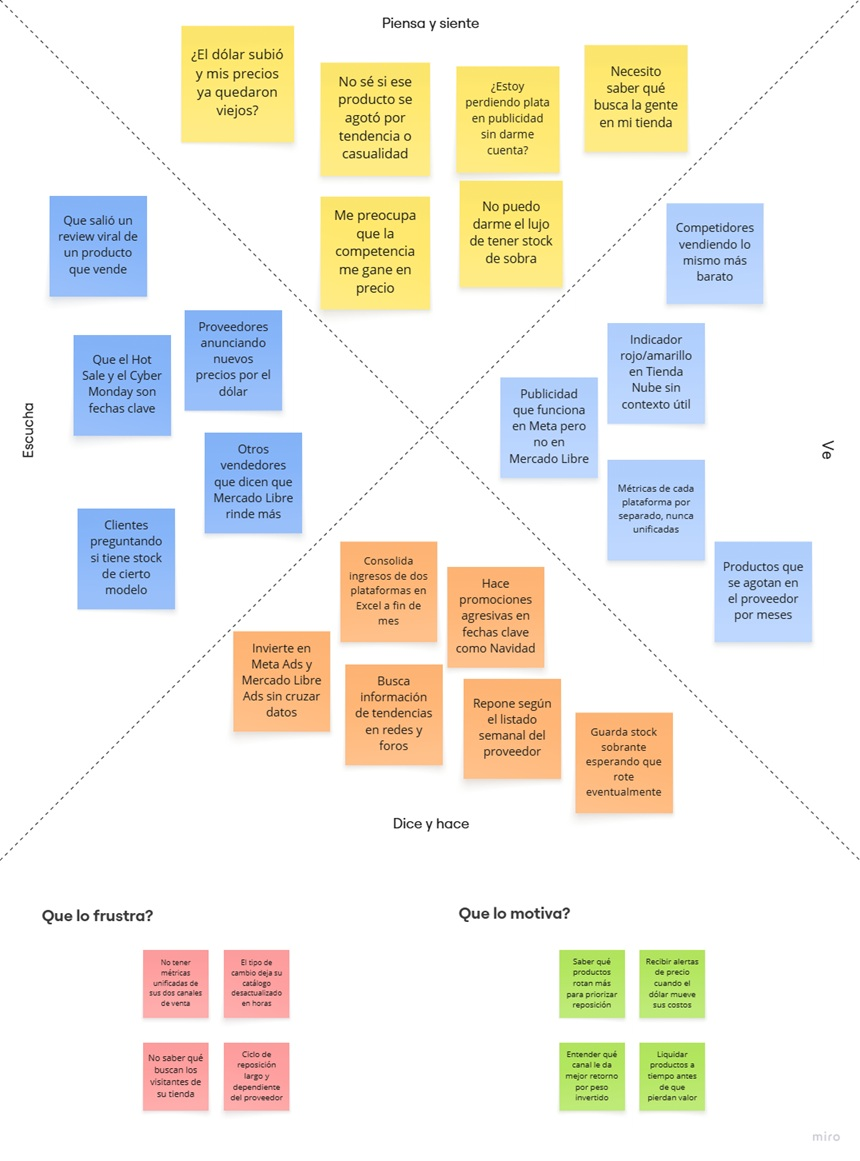
\includegraphics[width=\textwidth]{./images/mapa_empatia_nicolas_acosta.jpg}
    \caption{Mapa de empatía: Nicolás Acosta (rubro electrónica).}
    \label{fig:empatia-nicolas}
\end{figure}

\noindent\textit{Fuente: elaboración propia.}

\FloatBarrier

Los tres mapas convergen, cada uno desde la lógica particular de su rubro, en una misma tensión de fondo: información dispersa, en parte propia y en parte de la plataforma que utilizan, que ninguna de las tres personas logra traducir en una decisión oportuna. Esta convergencia refuerza, desde la síntesis cualitativa del Design Thinking, el mismo diagnóstico que la matriz FODA cruzado retoma a continuación con evidencia empírica adicional.

\section{Matriz FODA Cruzado}
\label{sec:foda-cruzado}

La matriz FODA (Fortalezas, Oportunidades, Debilidades y Amenazas) es una herramienta clásica de diagnóstico estratégico que organiza los factores internos y externos relevantes para un proyecto u organización. El análisis presentado a continuación no se limita, sin embargo, a la enumeración habitual de estos cuatro factores: se trata de una matriz FODA \emph{cruzado} (TOWS Matrix), en la que cada fortaleza y cada debilidad (factores internos) se combinan explícitamente con cada oportunidad y cada amenaza (factores externos) para generar cuatro tipos de estrategias derivadas (ofensivas, FO; adaptativas, DO; defensivas, FA; y preventivas, DA), en lugar de dejar dichos factores como una simple lista descriptiva \parencite{Weihrich1982}. La Figura~\ref{fig:foda-cruzado} presenta la matriz completa construida para el proyecto.

\begin{figure}[ht]
    \centering
    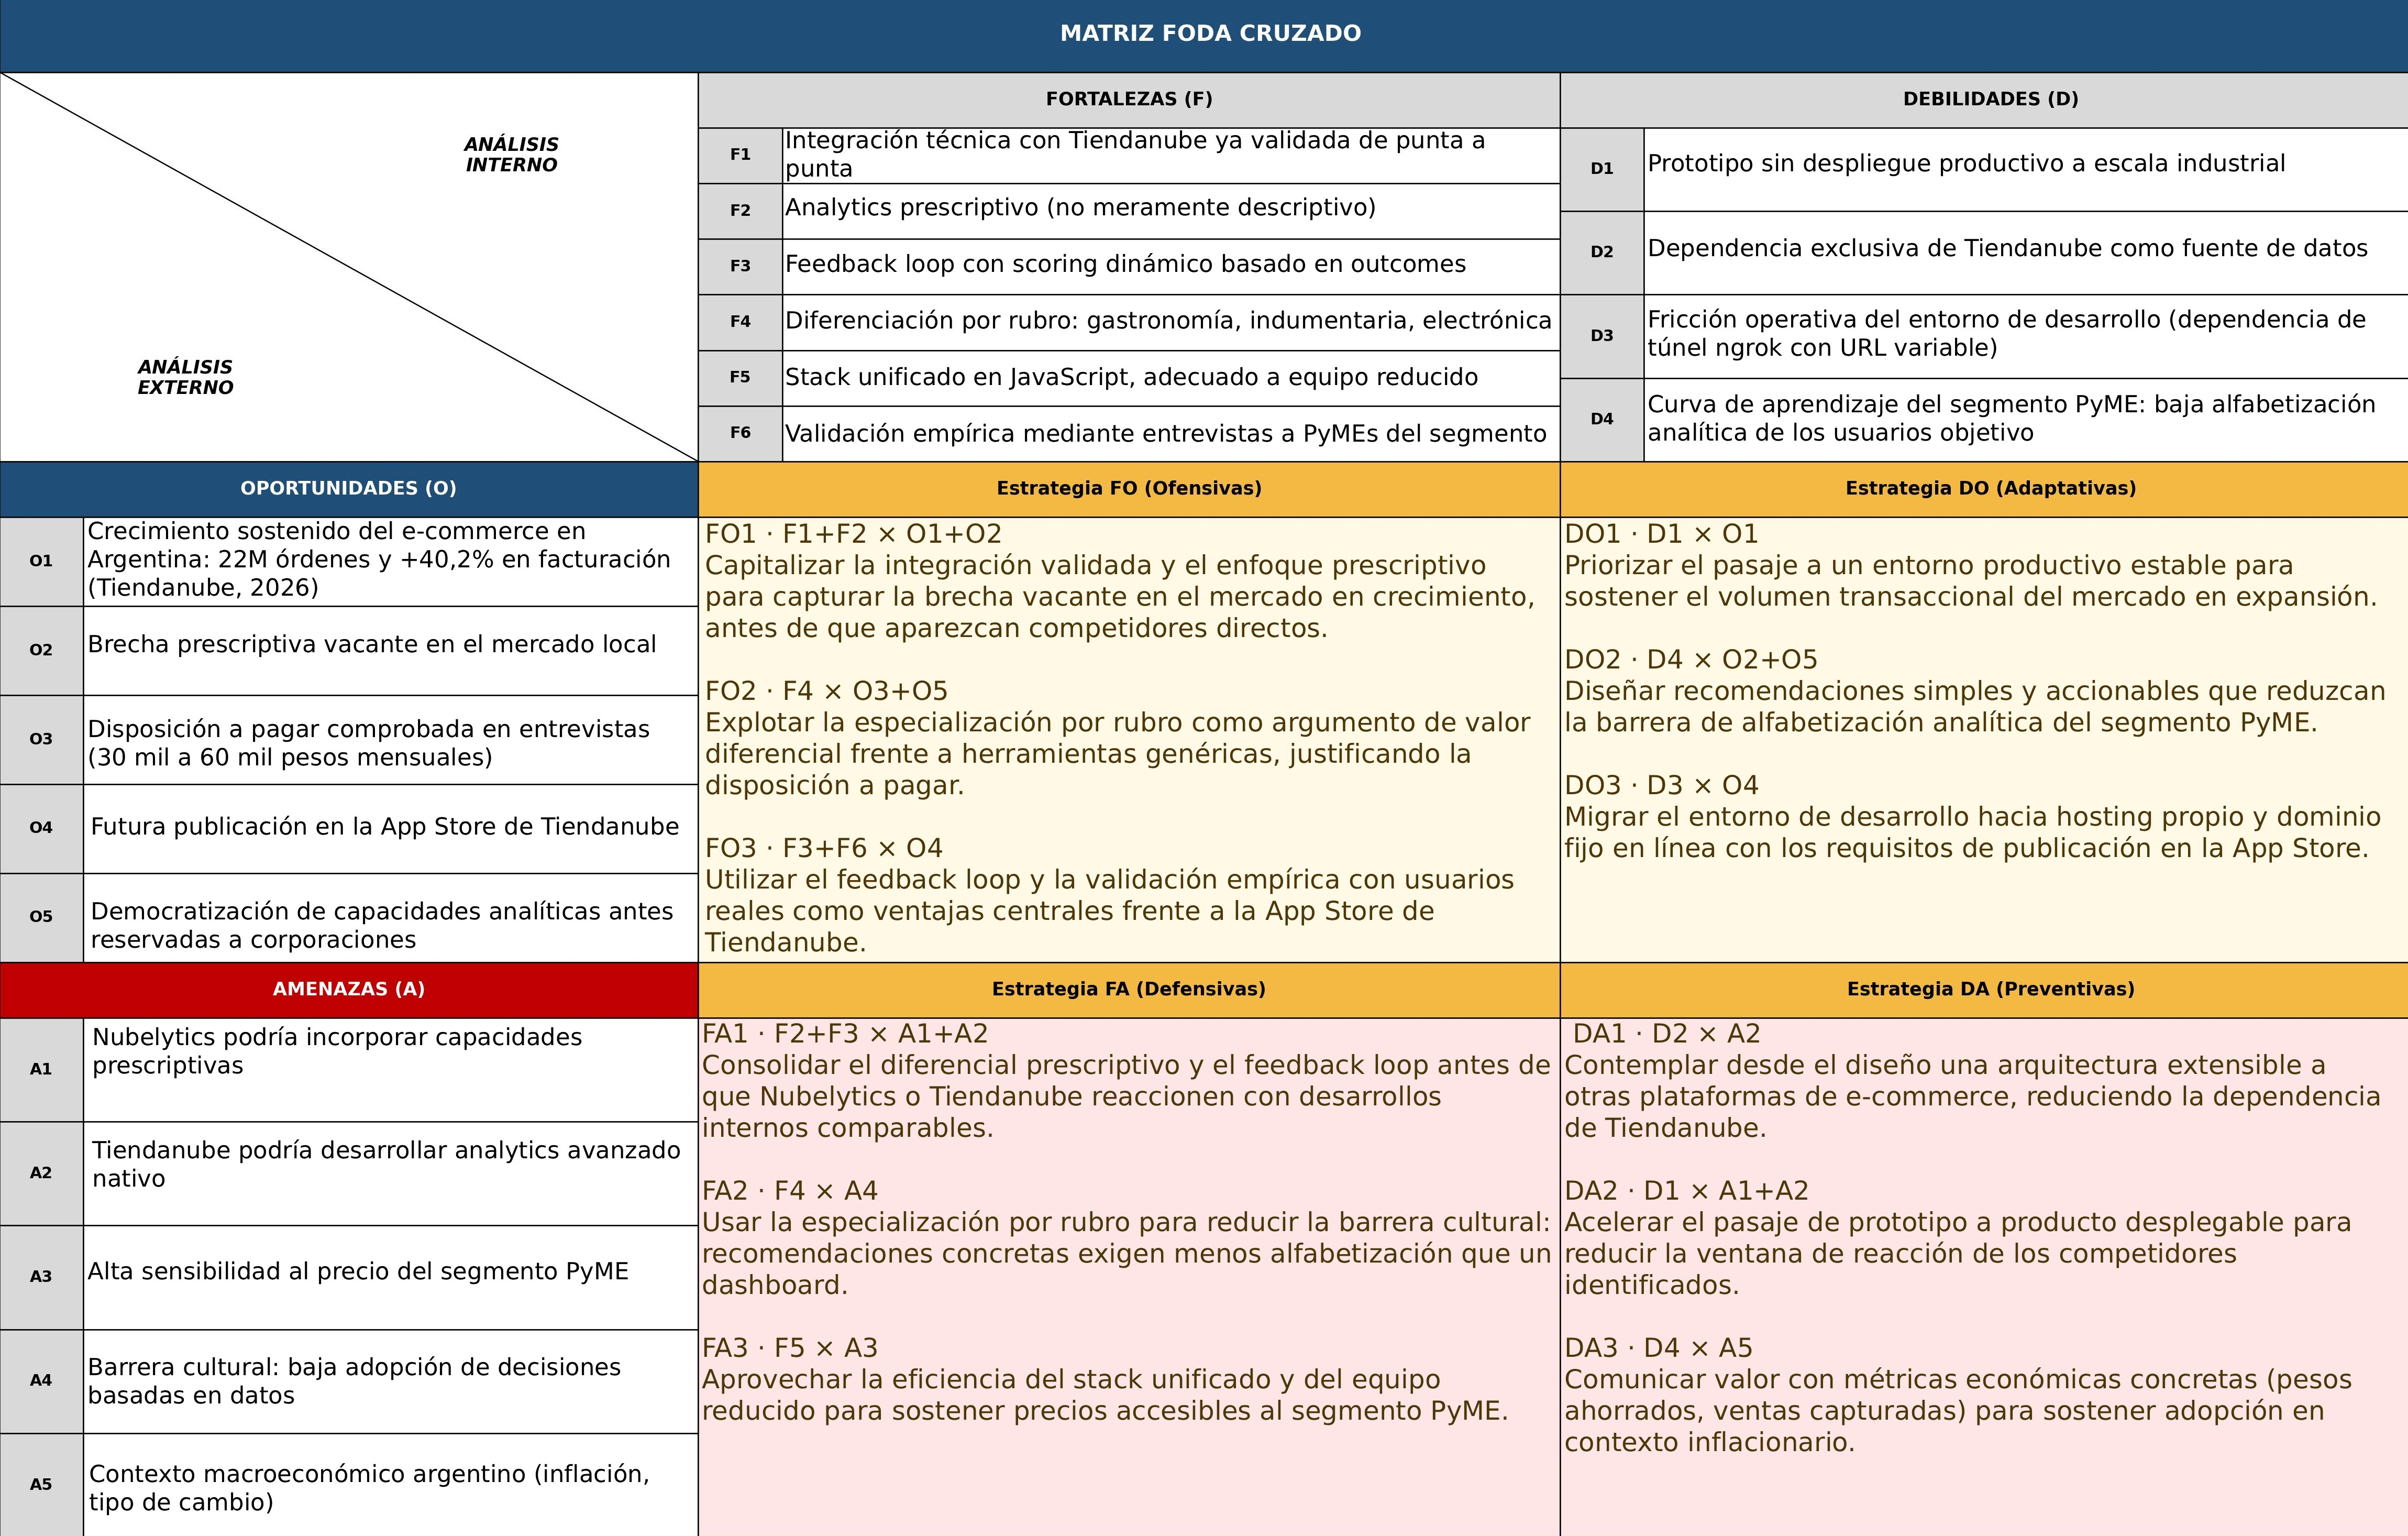
\includegraphics[width=\textwidth]{./images/foda_cruzado_decidata.jpg}
    \caption{Matriz FODA Cruzado del proyecto.}
    \label{fig:foda-cruzado}
\end{figure}

\noindent\textit{Fuente: elaboración propia.}

En el plano interno, las fortalezas identificadas se apoyan mayormente en decisiones técnicas ya descriptas y validadas en la sección~\ref{sec:stack-tecnologico}. La integración con Tiendanube fue validada de punta a punta (F1): la aplicación embebida carga correctamente dentro del panel de administración de la tienda de desarrollo, con el intercambio de Nexo funcionando de forma correcta entre el \emph{iframe} y la ventana padre, tal como se documentó en la sección~\ref{sec:arquitectura-red}. A esto se suma que el motor de análisis está orientado a un enfoque prescriptivo y no meramente descriptivo (F2), que incorpora un mecanismo de retroalimentación con scoring dinámico basado en outcomes (F3), que diferencia sus recomendaciones según el rubro comercial, gastronomía, indumentaria y electrónica (F4), que se apoya en un stack tecnológico unificado en JavaScript adecuado a un equipo reducido de dos personas, según los criterios de selección descriptos en la sección~\ref{sec:criterios-seleccion} (F5), y que fue validado empíricamente mediante entrevistas a comercios PyME del segmento objetivo, documentadas en el Anexo B (F6). En contraposición, las debilidades reconocidas remiten en su mayoría a limitaciones propias de un desarrollo en etapa de prototipo: el proyecto no contempla, por definición de alcance, un despliegue productivo a escala industrial (D1); depende de manera exclusiva de Tiendanube como única fuente de datos, sin integraciones a otras plataformas (D2); arrastra la fricción operativa señalada en la sección~\ref{sec:tunel-ngrok} respecto de la dependencia de un túnel de ngrok cuya URL pública cambia en cada reinicio (D3); y enfrenta una curva de aprendizaje propia del segmento PyME, cuyos usuarios objetivo presentan una alfabetización analítica baja (D4), tal como se observó de manera recurrente en las entrevistas del Anexo B.

En el plano externo, las oportunidades identificadas describen un mercado en expansión con una brecha metodológica concreta. El comercio electrónico argentino atraviesa un crecimiento sostenido: durante 2025 el ecosistema de Tiendanube alcanzó casi 22 millones de órdenes, con una facturación un 40,2\% superior a la inflación acumulada \parencite{Tiendanube2026} (O1). Dentro de ese mercado en expansión, el relevamiento de la sección 3 permitió identificar una brecha prescriptiva vacante (O2): ninguna de las herramientas accesibles localmente supera el nivel descriptivo, mientras que las soluciones internacionales con capacidades prescriptivas, descriptas en la sección 3.4, resultan incompatibles con la realidad del segmento PyME argentino. Esa brecha convive, además, con una disposición a pagar comprobada empíricamente en las entrevistas del Anexo B, con montos que oscilan entre los 30 mil y los 60 mil pesos mensuales según el perfil del comercio (O3), con la posibilidad futura de publicación formal en la tienda de aplicaciones de Tiendanube (O4) y con la oportunidad más amplia de democratizar, para comercios de pequeña escala, capacidades analíticas hasta ahora reservadas a estructuras corporativas (O5). Frente a estas oportunidades, las amenazas identificadas provienen tanto de la posible reacción de actores ya presentes en el mercado como de condiciones estructurales del segmento: Nubelytics, el antecedente local más próximo descripto en la sección 3.3, podría incorporar capacidades prescriptivas a su oferta actual (A1), y la propia Tiendanube podría desarrollar analítica avanzada de manera nativa dentro de su plataforma (A2); a esto se suman la alta sensibilidad al precio propia del segmento PyME (A3), la barrera cultural que supone la baja adopción de decisiones basadas en datos (A4) y el contexto macroeconómico argentino, marcado por la inflación y la volatilidad del tipo de cambio (A5).

El cruce sistemático de estos factores deriva en cuatro tipos de estrategias. Las estrategias ofensivas (FO), que combinan fortalezas con oportunidades para maximizarlas, priorizan capitalizar la integración ya validada con Tiendanube y el enfoque prescriptivo para capturar la brecha vacante en un mercado en crecimiento antes de que aparezcan competidores directos (FO1), y explotar la diferenciación por rubro como argumento de valor frente a herramientas genéricas para justificar la disposición a pagar relevada en las entrevistas (FO2). Esta última estrategia encuentra respaldo empírico directo en los montos concretos declarados por los propios comerciantes: Delfina Fernández, dueña de un emprendimiento de indumentaria bordada, indicó que pagaría entre 40 mil y 50 mil pesos mensuales por una herramienta de este tipo (Anexo B, Entrevista B.1); Morena Cejas, también del rubro indumentaria, situó ese valor entre 50 mil y 60 mil pesos (Anexo B, Entrevista B.2); Shakira, dueña de After Trash, se mostró dispuesta a pagar hasta 30 mil pesos mensuales siempre que pudiera validar previamente la herramienta mediante una prueba gratuita (Anexo B, Entrevista B.5); y Julián Fabbi, del rubro de venta de cómics y mangas, estimó un adicional de entre 5 mil y 10 mil pesos por sobre lo que ya paga a Tiendanube (Anexo B, Entrevista B.4). Las estrategias adaptativas (DO), que combinan debilidades con oportunidades para reducirlas, priorizan el pasaje hacia un entorno productivo estable que permita sostener el volumen transaccional de un mercado en expansión (DO1) y el diseño de recomendaciones simples y directamente accionables que reduzcan la barrera de alfabetización analítica propia del segmento PyME (DO2), una necesidad que se manifestó de forma recurrente en las entrevistas: Delfina Fernández reconoció no saber \enquote{qué tanto uso Tienda Nube} en la parte de datos (Anexo B, Entrevista B.1), mientras que Shakira planteó explícitamente que una alerta automática que le indicara cuándo sus precios quedaron desactualizados \enquote{sería ideal} (Anexo B, Entrevista B.5), validando la necesidad de recomendaciones prescriptivas por sobre reportes que requieran interpretación. Las estrategias defensivas (FA), que combinan fortalezas con amenazas para neutralizarlas, priorizan consolidar el diferencial prescriptivo y el mecanismo de retroalimentación antes de que Nubelytics o Tiendanube reaccionen con desarrollos internos comparables (FA1), y aprovechar la eficiencia del stack unificado y del equipo reducido para sostener precios accesibles frente a la sensibilidad al precio del segmento (FA3), una sensibilidad que también se refleja en las entrevistas: Morena Cejas condicionó explícitamente su disposición a pagar al impacto directo en ventas (\enquote{si me sirve en ventas... la pago}, Anexo B, Entrevista B.2), y Julián Fabbi ató el monto que pagaría de forma directamente proporcional al plan de Tiendanube que ya abona (Anexo B, Entrevista B.4). Finalmente, las estrategias preventivas (DA), que combinan debilidades con amenazas para minimizarlas, plantean contemplar desde el diseño una arquitectura extensible a otras plataformas de e-commerce que reduzca la dependencia exclusiva de Tiendanube (DA1) y comunicar el valor de la herramienta mediante métricas económicas concretas, pesos ahorrados, ventas capturadas, que resulten legibles en un contexto inflacionario (DA3). Esta última estrategia resulta particularmente pertinente a la luz de un episodio relatado por Shakira, quien vendió mercadería por 35 millones de pesos esencialmente al costo, sin margen de ganancia, por no haber actualizado a tiempo sus precios frente a la suba del dólar y de los insumos (Anexo B, Entrevista B.5): el problema concreto que este incidente ilustra es, precisamente, el tipo de situación que una recomendación prescriptiva oportuna busca prevenir, y comunicar la herramienta en esos términos económicos concretos, evitar pérdidas de esa magnitud, resulta más persuasivo para el segmento que una descripción abstracta de sus capacidades analíticas.

\section{Cinco Fuerzas de Porter}
\label{sec:porter}

El modelo de las cinco fuerzas de Porter permite evaluar la intensidad competitiva de un sector y, en consecuencia, su atractivo relativo para un nuevo participante, a partir del análisis de cinco dimensiones: la rivalidad entre competidores existentes, la amenaza de nuevos entrantes, el poder de negociación de los proveedores, el poder de negociación de los clientes y la amenaza de productos sustitutos \parencite{Porter1979}. La Figura~\ref{fig:porter} sintetiza la intensidad relevada para cada una de estas fuerzas en el contexto específico del presente proyecto.

\begin{figure}[ht]
    \centering
    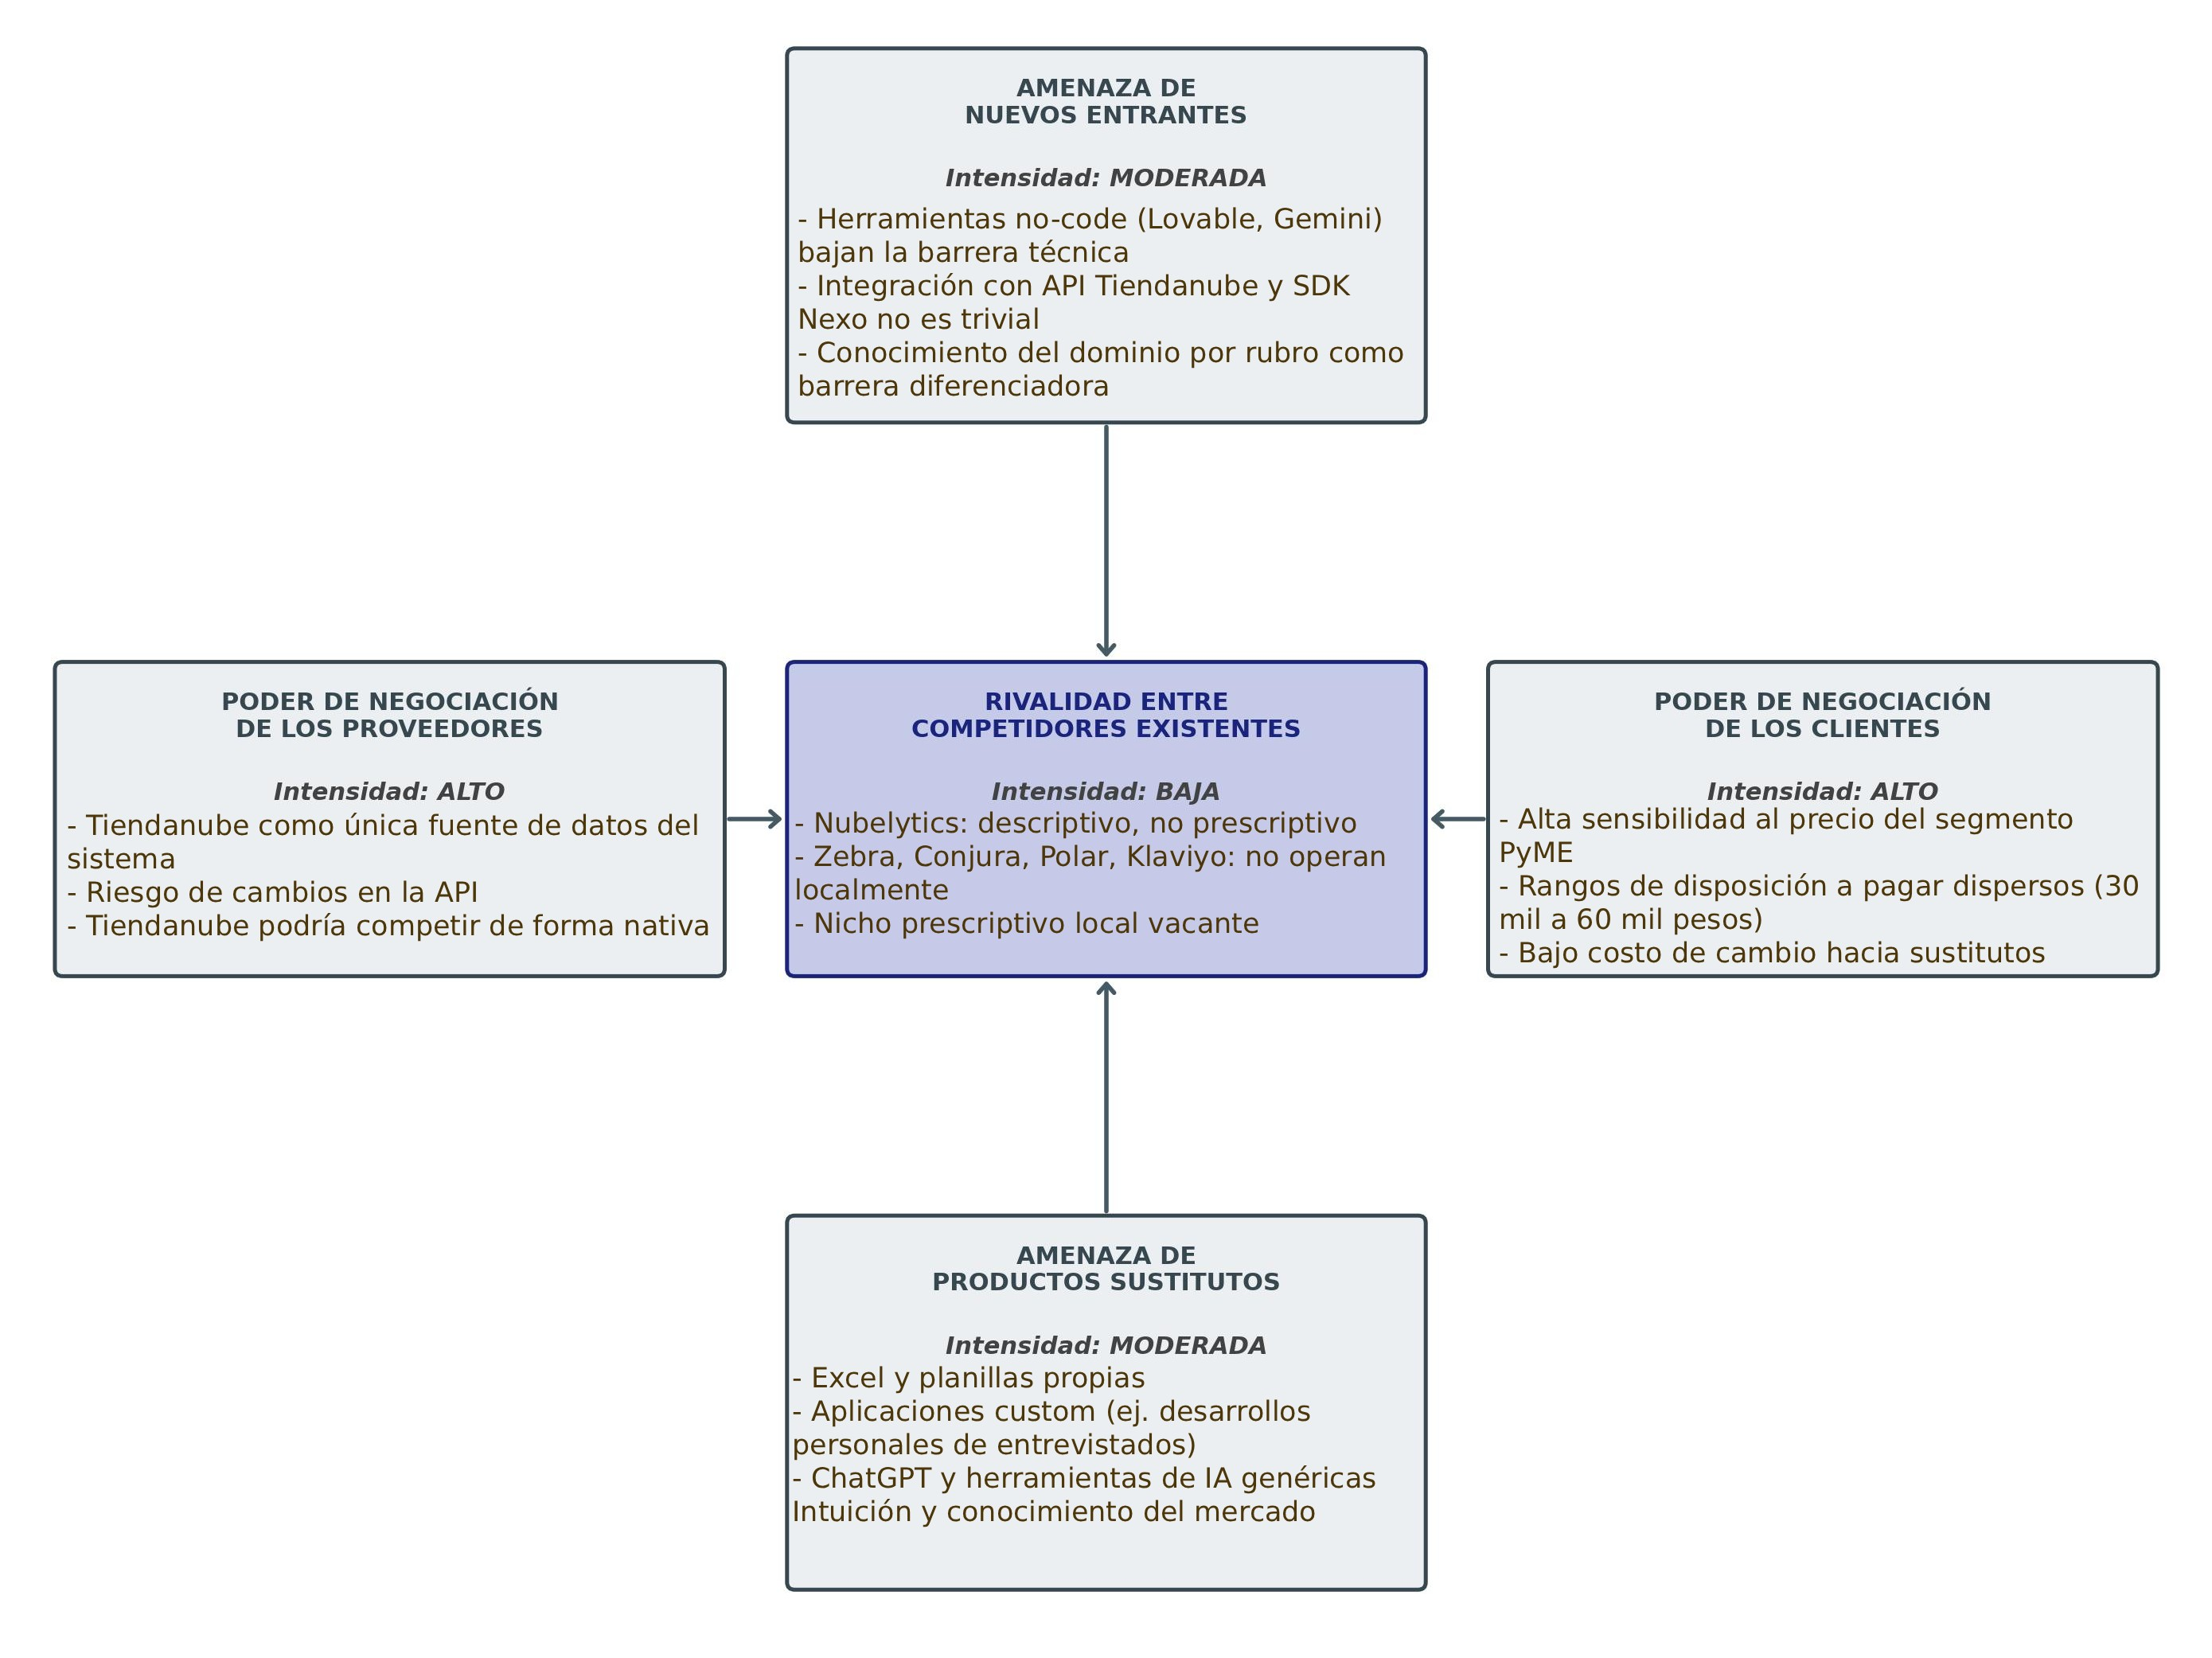
\includegraphics[width=\textwidth]{./images/porter_decidata.jpg}
    \caption{Cinco Fuerzas de Porter aplicadas al proyecto.}
    \label{fig:porter}
\end{figure}

\noindent\textit{Fuente: elaboración propia.}

La rivalidad entre los competidores existentes se evalúa como baja. Tal como se desarrolló en la sección 3, Nubelytics, el antecedente local más próximo, opera bajo un paradigma descriptivo y no prescriptivo (sección 3.3), mientras que las soluciones internacionales con capacidades prescriptivas, entre ellas Zebra Technologies, Conjura, Polar Analytics y Klaviyo, no operan localmente y presentan barreras de idioma, costo y adecuación al mercado latinoamericano que las vuelven inaccesibles para el segmento PyME argentino (sección 3.4). El nicho prescriptivo local, en consecuencia, permanece vacante, lo que reduce sustancialmente la presión competitiva directa sobre el proyecto en esta etapa.

La amenaza de nuevos entrantes se considera moderada. Por un lado, la proliferación de herramientas de desarrollo asistido por Inteligencia Artificial y de plataformas no-code, como Lovable o Gemini, reduce de manera concreta la barrera técnica para construir soluciones de analítica a medida sin necesidad de un equipo de desarrollo tradicional. Esta dinámica no es hipotética: Pablo Terrera, dueño de la cafetería MariCafé y con experiencia previa en analítica corporativa, construyó por su cuenta un sistema integral de analytics propio (\enquote{Maricapp}) combinando Lovable, Google Sheets y Gemini AI, replicando funcionalidades de proyección de ventas y control de egresos que en un contexto corporativo requerirían un equipo dedicado (Anexo B, Entrevista B.3). Por otro lado, dos factores actúan como barrera frente a esta amenaza: la integración con la API de Tiendanube y con el SDK Nexo no resultó trivial en la práctica, tal como se documentó en la sección~\ref{sec:frontend-react-vite} al describir los ajustes de configuración requeridos para conciliar Nexo y Vite con las restricciones del navegador, y el conocimiento específico de cada rubro comercial, en el que se apoya la diferenciación del proyecto (F4), constituye una barrera adicional que un desarrollo genérico con herramientas no-code no reproduce de forma inmediata.

El poder de negociación de los proveedores se evalúa como alto, dado que el proyecto depende de un único proveedor de datos: la API de Tiendanube constituye la fuente exclusiva de información sobre la que opera el motor de análisis, tal como se describió al detallar el stack tecnológico en la sección~\ref{sec:stack-tecnologico}. Esta dependencia expone al proyecto a dos riesgos concretos: cambios unilaterales en la API que podrían requerir modificaciones no planificadas en la capa de integración, y la posibilidad, ya contemplada como amenaza A2 en la matriz FODA cruzado, de que la propia Tiendanube decida competir de forma nativa ofreciendo analítica avanzada dentro de su plataforma, un escenario ante el cual el proyecto carecería de capacidad de negociación.

El poder de negociación de los clientes también se evalúa como alto, en el segmento de las PyMEs y emprendimientos de e-commerce en Argentina, caracterizado por una fuerte sensibilidad al precio y por costos de cambio comparativamente bajos hacia alternativas. Las propias entrevistas documentan esta dinámica: Morena Cejas dejó de pagar el plan pago de Tiendanube al no percibir un rendimiento proporcional a su costo, y redirigió ese presupuesto a publicidad (Anexo B, Entrevista B.2), mientras que Shakira migró la totalidad de su tienda de Tiendanube hacia Tienda Negocio, una plataforma más económica y sin comisión por venta (Anexo B, Entrevista B.5). Ambos casos ilustran que los comercios del segmento objetivo están dispuestos a discontinuar o migrar servicios pagos cuando no perciben valor proporcional a su costo, lo que se traduce en rangos de disposición a pagar dispersos, entre 30 mil y 60 mil pesos mensuales según se detalló en la sección~\ref{sec:foda-cruzado}, y en la necesidad de demostrar valor de forma temprana y concreta para sostener la adopción.

La amenaza de productos sustitutos se evalúa como moderada. Ningún comerciante entrevistado depende exclusivamente de las herramientas nativas de su plataforma de e-commerce para gestionar su negocio: todos recurren, en mayor o menor medida, a sustitutos propios. Delfina Fernández registra sus ventas y su proceso de producción en una aplicación a medida desarrollada por un colaborador (Anexo B, Entrevista B.1); Morena Cejas lleva el control de stock y costos en Excel, con la asistencia de su padre (Anexo B, Entrevista B.2); Julián Fabbi consolida en Excel los ingresos de sus dos canales de venta porque Tiendanube no contempla ciertos valores que necesita (Anexo B, Entrevista B.4); Pablo Terrera reemplazó por completo el registro en papel y planillas por su sistema propio Maricapp (Anexo B, Entrevista B.3); y Shakira utiliza ChatGPT de forma constante para analizar datos, redactar comunicaciones y pensar estrategias, al punto de describirlo como \enquote{mi socio} (Anexo B, Entrevista B.5). A estos sustitutos digitales se suma, en todos los casos, la intuición y el conocimiento acumulado del propio negocio como mecanismo de decisión de facto. Esta diversidad de sustitutos limita el poder de una única solución para imponerse de forma inmediata, aunque su naturaleza fragmentada y manual, antes que la existencia de un competidor prescriptivo consolidado, es lo que mantiene esta amenaza en un nivel moderado y no alto.

La lectura conjunta de las cinco fuerzas describe un mercado de atractivo relativo alto para el proyecto: la rivalidad directa es baja y la amenaza de sustitutos, aunque presente, es fragmentaria y no consolidada, lo que deja margen para una propuesta prescriptiva diferenciada. La principal tensión competitiva no proviene, en consecuencia, de otros actores ofreciendo hoy una solución equivalente, sino de la concentración del poder de negociación en los extremos de la cadena: en el proveedor único de datos, Tiendanube, y en un segmento de clientes con alta sensibilidad al precio y bajo costo de cambio. Esa tensión es la que las estrategias defensivas y preventivas derivadas de la matriz FODA cruzado, desarrolladas en la sección~\ref{sec:foda-cruzado}, buscan mitigar.

\section{Estrategia comercial: Triple P}
\label{sec:triple-p}

El FODA cruzado desarrollado en la Sección~\ref{sec:foda-cruzado} y las cinco fuerzas de Porter analizadas en la Sección~\ref{sec:porter} evaluaron la viabilidad competitiva del proyecto: qué tan favorable es el entorno externo y qué tan sólidas son las capacidades internas para capturarlo. Ninguno de los dos marcos formaliza, sin embargo, cómo el proyecto se posiciona comercialmente frente al segmento objetivo, es decir, qué se ofrece, a qué precio y a través de qué canal se distribuye y se comunica esa oferta. El análisis de marketing mix o Triple P (Producto, Precio, Plaza y Promoción) cubre ese vacío: traduce en una estrategia comercial concreta los cinco atributos diferenciales identificados en la comparación con el estado del arte (Sección 3.5), con énfasis particular en la accesibilidad financiera, uno de esos cinco atributos que, a diferencia de los otros cuatro, no había sido desarrollado todavía en este capítulo. La Figura~\ref{fig:triple-p} sintetiza los tres ejes de esa estrategia.

\begin{figure}[ht]
    \centering
    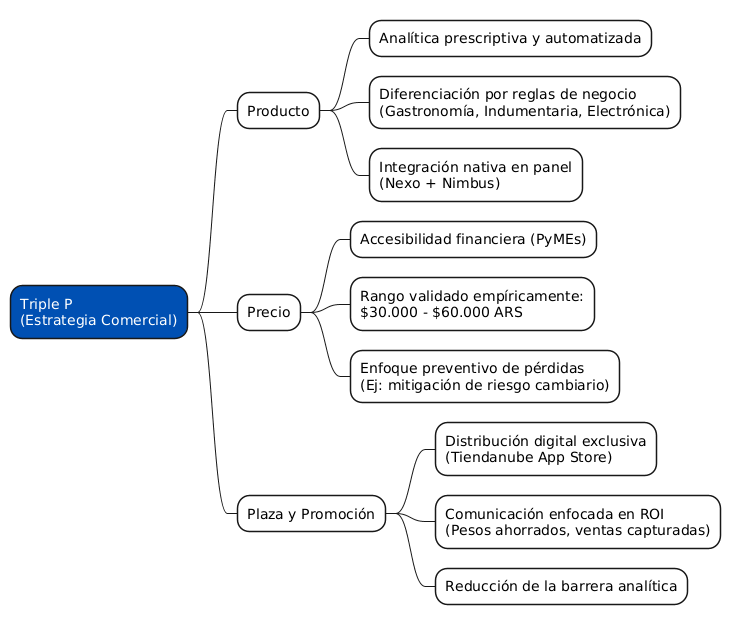
\includegraphics[width=0.85\textwidth]{./images/diagramaTripleP.png}
    \caption{Estrategia comercial Triple P del proyecto.}
    \label{fig:triple-p}
\end{figure}

\noindent\textit{Fuente: elaboración propia.}

\subsection{Producto}
\label{sec:triple-p-producto}

El eje de producto se apoya en tres atributos ya fundamentados a lo largo de la tesis, que aquí se integran bajo una misma lógica comercial en lugar de repetir su desarrollo técnico. En primer lugar, el sistema ofrece analítica prescriptiva y automatizada, no meramente descriptiva: la distinción entre ambos niveles de madurez analítica se estableció en la Sección 2.2 del Marco Teórico y se validó frente al estado del arte en la Sección 3.5, donde se constató que ninguna de las herramientas accesibles localmente combina recomendaciones prescriptivas con accesibilidad para el segmento PyME argentino. En segundo lugar, el producto diferencia sus reglas de negocio según el rubro comercial, gastronomía, indumentaria y electrónica, caracterización descripta en la Sección 2.4 del Marco Teórico y formalizada en los requerimientos RF-06, identificación del rubro a partir del recurso \texttt{Store} de la API de Tiendanube, y RF-10, reglas de detección de rotación decreciente diferenciadas por rubro. Esta diferenciación no es un detalle técnico secundario sino un argumento de producto: el sistema no ofrece un tablero genérico, sino reglas adaptadas al negocio concreto de cada comerciante. En tercer lugar, la integración nativa en el panel de administración de Tiendanube mediante el SDK Nexo y el sistema de diseño Nimbus (Sección~\ref{sec:frontend-react-vite}) elimina la fricción de adopción propia de una herramienta externa: el comerciante no necesita instalar, aprender ni acceder a una plataforma adicional, sino que la solución aparece integrada al entorno donde ya opera su tienda.

\subsection{Precio}
\label{sec:triple-p-precio}

El eje de precio desarrolla el atributo señalado como ausente hasta este punto del capítulo: la accesibilidad financiera, uno de los cinco atributos diferenciales definidos en la Sección 3.5 frente a las soluciones internacionales de analítica prescriptiva, cuyos costos en moneda extranjera resultan, según se documentó en esa sección, incompatibles con la realidad del segmento PyME argentino.

La disposición a pagar del segmento objetivo fue validada empíricamente en las entrevistas del Anexo B y ya se citó de forma puntual en la estrategia FO2 de la Sección~\ref{sec:foda-cruzado}: Delfina Fernández declaró un rango de 40 mil a 50 mil pesos mensuales (Anexo B, Entrevista B.1); Morena Cejas, de 50 mil a 60 mil pesos (Anexo B, Entrevista B.2); Shakira, hasta 30 mil pesos mensuales (Anexo B, Entrevista B.5); y Julián Fabbi, un adicional de 5 mil a 10 mil pesos por sobre lo que ya paga a Tiendanube (Anexo B, Entrevista B.4). La dispersión entre estos montos, de un adicional marginal de 5 mil pesos a un compromiso pleno de 60 mil, no es ruido estadístico sino una señal comercial: la disposición a pagar depende directamente de la percepción de valor y del punto de partida de cada comercio, y no admite un precio único ni una comunicación homogénea para todo el segmento.

Dentro de esa dispersión, el caso de Shakira introduce una condición que los demás entrevistados no plantearon de forma explícita: su disposición a pagar hasta 30 mil pesos está supeditada a validar previamente la herramienta mediante una prueba gratuita. Consultada de forma directa sobre un período de prueba, respondió: \enquote{Sí, totalmente. Si en el período de prueba me muestra algo útil que yo no estaba viendo, ahí me convence. La herramienta sola no alcanza; necesito ver el valor en la práctica} (Anexo B, Entrevista B.5). Esta condición, sumada a la reticencia de Morena Cejas a comprometer un monto sin comprobar antes su impacto en ventas (Anexo B, Entrevista B.2), informa una estrategia de precio de tipo \emph{freemium} o con período de prueba gratuito: en un segmento con alta sensibilidad al precio y bajo costo de cambio, ya caracterizado como fuerza de negociación de clientes de intensidad alta en la Sección~\ref{sec:porter}, exigir el pago antes de demostrar el valor concreto de la herramienta constituye una barrera de adopción evitable.

Finalmente, el precio se comunica no como un costo sino como una prevención de pérdidas concretas. El episodio relatado por Shakira, quien vendió mercadería por 35 millones de pesos esencialmente al costo por no haber actualizado sus precios a tiempo frente a la suba del dólar y de los insumos (Anexo B, Entrevista B.5), ya citado como fundamento de la estrategia preventiva DA3 en la Sección~\ref{sec:foda-cruzado}, ilustra el argumento central de este enfoque: frente a una pérdida de esa magnitud, un costo mensual de entre 30 mil y 60 mil pesos no se percibe como un gasto sino como una prevención frente a un riesgo concreto y ya materializado para al menos una comerciante del segmento.

\subsection{Plaza y Promoción}
\label{sec:triple-p-plaza-promocion}

Los ejes de plaza y promoción se desarrollan de forma conjunta porque, en la estrategia del proyecto, ambos dependen de la misma decisión de fondo: distribuir y comunicar la herramienta dentro del mismo ecosistema donde el comerciante ya opera, en lugar de captarlo hacia una plataforma externa.

La distribución es exclusivamente digital, a través de la tienda de aplicaciones de Tiendanube (\emph{App Store}), señalada como la oportunidad O4 en la matriz FODA cruzado de la Sección~\ref{sec:foda-cruzado}. Esta decisión de plaza es consistente con el producto descripto en la Sección~\ref{sec:triple-p-producto}: al tratarse de una aplicación integrada mediante Nexo y Nimbus, su canal natural de distribución es el mismo directorio de aplicaciones donde el comerciante ya busca herramientas para su tienda, sin requerir una estrategia de adquisición independiente.

La promoción, por su parte, se enfoca en un retorno de inversión medible, pesos ahorrados, ventas capturadas, pérdidas evitadas, y no en una descripción abstracta de capacidades analíticas. Este enfoque retoma de forma directa la estrategia preventiva DA3 de la Sección~\ref{sec:foda-cruzado} y responde a una necesidad relevada explícitamente en las entrevistas del Anexo B: Morena Cejas condicionó su disposición a pagar al impacto directo en ventas (\enquote{si me sirve en ventas... la pago}, Anexo B, Entrevista B.2), y Shakira fue igual de explícita al señalar que \enquote{necesito ver que realmente sirve} antes de comprometerse (Anexo B, Entrevista B.5). Comunicar la herramienta en términos de resultados económicos concretos no es, a la luz de estos testimonios, una preferencia estilística sino una condición para que la propuesta resulte persuasiva para este segmento.

A esta comunicación centrada en resultados se suma una reducción explícita de la barrera analítica: el sistema no exige formación técnica para interpretar sus salidas, dado que cada recomendación se entrega en lenguaje natural (RNF-09) mediante la traducción automática de datos estructurados que ejecuta el backend a través de la API del proveedor de IA (RF-19, Sección~\ref{sec:generacion-mensajes-ia}). Esta característica es, en sí misma, un argumento de promoción: reduce la carga cognitiva que, según se relevó en la Sección~\ref{sec:metodologia-entrevistas}, constituye una de las principales fricciones del segmento objetivo frente a las herramientas analíticas existentes.

El análisis Triple P desarrollado en esta sección no introduce nuevos atributos diferenciales, sino que formaliza, desde una perspectiva estrictamente comercial, la misma propuesta de valor que la matriz FODA cruzado y las cinco fuerzas de Porter evaluaron desde las perspectivas competitiva y operativa. Los tres análisis convergen, en particular, en dos puntos: la centralidad de la accesibilidad financiera para un segmento con alta sensibilidad al precio y bajo costo de cambio, y la necesidad de comunicar el valor de la herramienta en términos económicos concretos y no meramente técnicos. La síntesis estratégica que cierra el capítulo, a continuación, integra estos tres análisis en un diagnóstico consolidado.

\section{Síntesis estratégica}
\label{sec:sintesis-estrategica}

El análisis desarrollado en este capítulo converge en un diagnóstico consistente desde dos marcos metodológicos independientes. La matriz FODA cruzado identifica que las fortalezas más relevantes del proyecto, la integración técnica ya validada, el enfoque prescriptivo y el mecanismo de retroalimentación, se cruzan de manera directa con una oportunidad de mercado concreta y medible: una brecha prescriptiva vacante en un mercado en expansión y con disposición a pagar comprobada empíricamente en el segmento. El modelo de las cinco fuerzas de Porter, por su parte, confirma ese diagnóstico desde una perspectiva competitiva: la rivalidad directa es baja y la amenaza de sustitutos es fragmentaria, lo que sostiene la existencia de una oportunidad real y no meramente teórica. Ambos marcos coinciden, asimismo, en señalar la misma fuente estructural de riesgo desde dos ángulos distintos: la dependencia exclusiva de Tiendanube como proveedor único de datos, que aparece tanto como debilidad interna (D2) como fuerza de negociación de proveedores de intensidad alta, y la sensibilidad al precio del segmento PyME, que aparece tanto como amenaza externa (A3) como fuerza de negociación de clientes de intensidad alta.

Esta convergencia refuerza, en lugar de modificar, la propuesta de valor diferencial identificada en la sección 3.5 a partir de la comparación con Nubelytics y con las soluciones internacionales de analítica prescriptiva. Los cinco atributos allí definidos como constitutivos de esa propuesta de valor, recomendaciones prescriptivas y accionables, adaptación por rubro comercial, integración nativa con la API de Tiendanube, accesibilidad técnica y financiera para el segmento PyME, y un mecanismo de retroalimentación en bucle cerrado, se corresponden de manera directa con las fortalezas cruzadas en las estrategias ofensivas (FO) de la sección~\ref{sec:foda-cruzado} y con los factores que explican la baja rivalidad competitiva relevada en la sección~\ref{sec:porter}. El análisis estratégico realizado en este capítulo no agrega, en consecuencia, nuevos atributos a esa propuesta de valor, sino que la valida desde una perspectiva metodológica distinta y la vincula explícitamente con evidencia empírica concreta: los montos de disposición a pagar declarados por los propios comerciantes entrevistados, los sustitutos manuales o fragmentarios que hoy utilizan en ausencia de una alternativa prescriptiva, y episodios concretos que ilustran de manera directa el costo de no contar con una herramienta de este tipo, como el de Shakira, cuya falta de una alerta oportuna sobre precios desactualizados le representó pérdidas por 35 millones de pesos.

En conjunto, el análisis estratégico presentado en este capítulo sostiene que el proyecto no solo cubre una vacante metodológica en el estado del arte, sino que se posiciona en condiciones estructuralmente favorables para capturarla: opera en un mercado de bajo atractivo para competidores directos, cuenta con fortalezas técnicas ya validadas y dispone de evidencia empírica temprana que respalda tanto la existencia del problema que busca resolver como la disposición del segmento objetivo a pagar por su solución. Los principales riesgos identificados, la dependencia de un proveedor único de datos y la sensibilidad al precio del segmento, no invalidan esta conclusión, pero sí delimitan con precisión las prioridades a atender en las etapas siguientes del proyecto, en particular en lo referido a la extensibilidad de la arquitectura y a la comunicación del valor económico concreto de la herramienta.
